\section{Proposition} \label{chapter4:proposition}

This thesis proposes a platform allowing a seamless shift of focus to follow the development of a web application from the productivity required in the early beginning until the efficiency required during maturation.

Developers start a project without compromises on productivity.
The language targets an event-driven execution model.
And they continuously transform their implementation to target the more efficient pipeline architecture.

% The proposed platform allows to develop applications targeting an event-driven platform allowing productivity, and transforms them so as to execute them on a pipeline architecture allowing efficiency.
% It is based on the transformation of an event-driven program to target a pipeline architecture.

% The event-driven platform is embodied by Javascript for the implementation of this thesis.
% \textit{Node.js} is an efficient event-driven execution model to implement a web application.
% Javascript features higher-order programming, dynamic typing and a global memory abstraction.
% Because of these features, it is very productive.
% It makes Javascript a language of choice to develop web applications.

\textit{Node.js} implements Javascript, a productivity language, with an event driven execution model to implement web applications with decent performances.
However, the performance of this execution model is limited by the sequentiality of execution required to preserve exclusivity of memory accesses.
The pipeline execution model overstep this performance limitation.
It enforces memory isolation between stages allowing the parallel execution required for efficiency.
But this isolation limits the productivity because it avoids higher-order programming.
The difference in the memory abstractions between the two execution models is illustrated in figure \ref{fig:difference}.

\begin{figure}[h!]
\begin{center}
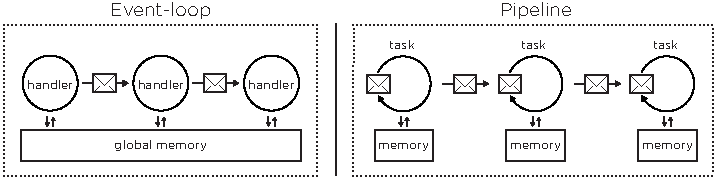
\includegraphics[width=0.9\textwidth]{../resources/models-difference.pdf}
\end{center}
\caption{Differences of memory abstraction}
\label{fig:difference}
\end{figure}


% \subsection{Equivalence}
% The difference of memory model between the two execution model is illustrated in figure \ref{fig:mem-equivalence}.
Despite this difference, these two execution models present an interesting similarity.
They both organize the execution as a sequence of tasks causally scheduled. %, as illustrated in figure \ref{fig:run-equivalence}.
This thesis proposes an equivalence between these two execution models based on this similarity.
Following this equivalence, it proposes a compiler that distributes the global memory into isolated stages of the pipeline.
% with message passing.
% As explained below, the concurrency model of the event-loop execution model, and the parallel approach of the pipeline execution model are very similar.
Concretely, it transforms a mono-threaded, event-driven application to run on a parallel pipeline architecture.

\subsection{Continuous Development}

%It proposes this equivalence as a solution to allow the same platform to propose a continuity of compromises between productivity and efficiency.
This transformation allows a continuity of compromises between productivity and efficiency to seamlessly follow the shift of focus during development.

% Developers keep two organizations of the implementations of an application.
% The organization based on event-driven execution model assures productivity whereas the transformation targeting the pipeline architecture helps improve efficiency.




% Developers keep two organizations of the implementation of an application. %, allowing them to start with productivity, and seamlessly abandon it for efficiency as the project matures.
% The productive organization is based on the event-driven execution model.
% It helps to maintain the application.
% The efficient organization is the transformed application targeting the pipeline execution model.

At first, the focus remains on the productivity of development rather than the efficiency of execution.
The development begins with the event-driven model to take advantage of the productivity of the global memory abstraction.
% and the asynchronous control flow of the event-driven execution model.
The execution resulting from the transformation is as efficient as the original event-driven execution model.

During the maturation of the application, the focus continuously shift towards efficiency.
The transformation distribute the global memory into isolated stages as much as possible.
It allows developer to identify the dependencies in this global memory avoiding the distribution.
They can identify these dependencies, and arrange the implementation accordingly to allow parallelism.
It helps developers to enforce efficiency through continuous iteration, instead of disruptive shifts of technology.

% The next paragraphs introduce this equivalence.


% \begin{figure}[h!]
% \begin{center}
% 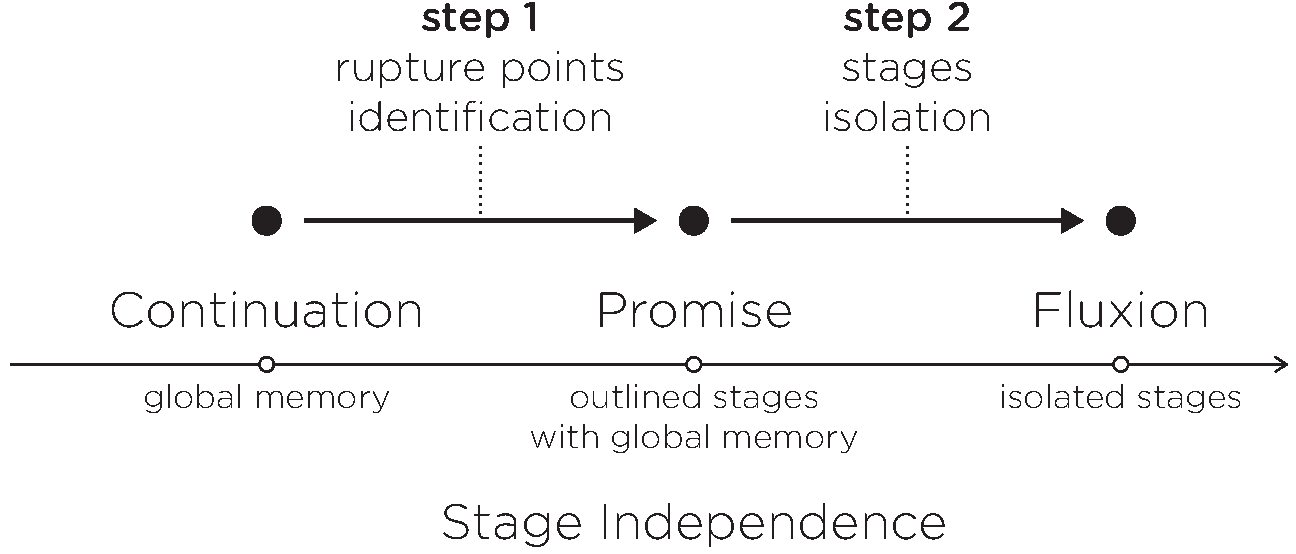
\includegraphics[width=0.7\textwidth]{../resources/roadmap.pdf}
% \end{center}
% \caption{Roadmap}
% \label{fig:roadmap}
% \end{figure}

\subsection{Equivalence} \label{chapter4:equivalence}

% The goal of this thesis is not to propose a new high-level language but to automate the architectural shift.
% The next paragraphs introduces the equivalence
The equivalence between these two execution models is broken down in two steps. %, as illustrated in figure \ref{fig:roadmap}.
The first step identifies the stages in the control flow, by detecting rupture points between them.
% The first step identifies the rupture points in the control flow separating the stages of the pipeline.
The second step enforces isolation of memory between these stages, and replaces synchronization with message passing to preserve the invariance.
% invariance through message passing.

\subsubsection{Execution Independence}

\begin{wrapfigure}{r}{0.33\textwidth}
  \vspace{-10pt}
  \begin{center}
    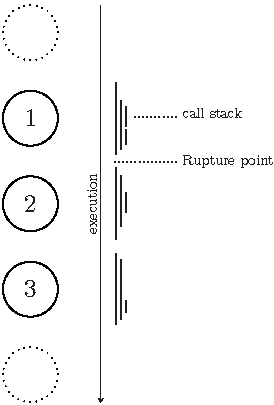
\includegraphics[height=0.4\textwidth]{../resources/rupture-point.pdf}
    \caption{Rupture point}
    \label{fig:rupture-point}
  \end{center}
  \vspace{-10pt}
\end{wrapfigure}

% The pipeline architecture enforces the memory isolation between stages.
In the pipeline architecture, each stage has its own thread of execution independent from the others.
Whereas in the event-driven execution model, the handlers are executed sequentially.
% the execution flow jumps from one concurrent handler to the other to execute them sequentialy.
%  because of the continuation passing style and the common memory store.
% The message passing linking the callbacks is transparently handled by the event-loop.
Despite this difference, the execution of a handler is as independent as the execution of a stage of a pipeline.
The call stacks of two handlers are isolated, as illustrated in figure \ref{fig:rupture-point}.
Indeed, a handler holds the execution until its call stack is empty, when all synchronous function calls terminates. Only then it yields the execution to the event-loop, which schedule the next handler.
A rupture point separates the call stacks of two handlers.



\subsubsection{Rupture points} \label{chapter5:flx-compiler:analyzer:rupture}

A rupture point is a call of a loosely coupled function.
It is an asynchronous call without subsequent synchronization with the caller.
This asynchronous function call is equivalent to a data-flow between two stages in the pipeline architecture.
The parent sends a message to the child handler containing the result of the asynchronous function call it initiated.
The event-driven execution model expects callback to send the message and continue the execution once the asynchronous call completes.

\paragraph{Callbacks, Listeners and Continuations}

A callback is a function passed as a parameter to a function call.
It is not inherently asynchronous.
Only two kinds of callbacks are asynchronous, listeners and continuations.
They are invoked to continue the execution with data not yet available synchronously, in the caller context.
Listeners listen to a stream of events, hence are invoked multiple times.
Whereas continuations are invoked only once to continue the execution after an asynchronous operation completes.
The two corresponding types of rupture points are \textit{start} and \textit{post}.

\textbf{Start rupture points} (listeners) are on the border between the application and the outside, continuously receiving incoming user requests.
An example of a start rupture point is in listing \ref{lst:source}, between the call to \texttt{app.get()}, and its listener \texttt{handler}.
These rupture points indicate the input of a data stream in the program, and the beginning of a chain of fluxions to process this stream.

\textbf{Post rupture points} (continuations) represent a continuity in the execution flow after an asynchronous operation yielding a unique result, such as reading a file, or a database.
An example of a post rupture points is in listing \ref{lst:source}, between the call to \texttt{fs.readFile()}, and its continuation \texttt{reply}.




% The rupture between the call stacks of two handlers is indicated by an asynchronous function call in the parent handler defining a children handler as a continuation or a listener.
% The asynchronous function call - the callee - between the caller and its continuation represents a rupture between the two call stacks.
% And the call stack of the continuation is independent from the call stack of the caller and the callee.

% TODO Definition of the two types of rupture points

% Both the pipeline architecture and the event-loop present these rupture points.
The detection of rupture points allows to retrieve the data-flow and the stages for a pipeline architecture from the implementation following the event-loop model.
% To allow the transformation from one to the other,
% The proposed platform detects rupture points defining stages. %, and distributes the global memory into them.
The implementation of this detection is fully addressed in the next chapter, in sections \ref{chapter5:due:compiler} and \ref{chapter5:flx:compiler}.
% It presents the extraction of a pipeline of concurent tasks from a Javascript application.
% Such pipeline is similar to the one exposed by Promises.
% The chapter proposes a simpler alternative to the latter called Dues.
However, these stages still require a global memory to communicate.
They can't be executed in parallel without breaking the invariance.





\subsubsection{Invariance}

% This transformation is important on two points.
% The conservation of the invariance.
% The equivalence between the coordinations.

\begin{wrapfigure}{l}{0.5\textwidth}
  \begin{minipage}[t]{0.20\textwidth}
    \centering
    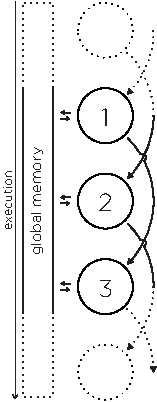
\includegraphics[page=1, height=2\linewidth]{../resources/invariance.pdf}
    \vfill
    \caption{Sequential scheduling}
    \label{fig:total-scheduling}
  \end{minipage}
  \hfill
  \vrule
  \hfill
  \begin{minipage}[t]{0.20\textwidth}
    \centering
    \includegraphics[page=2, height=2\linewidth]{../resources/invariance.pdf}
    \vfill
    \caption{Causal scheduling}
    \label{fig:causal-scheduling}
  \end{minipage}
\end{wrapfigure}

A global memory requires the sequential scheduling of handlers to assure exclusivity of access, as illustrated in figure \ref{fig:sequential-scheduling}. % which implies the total scheduling with a queue, as illustrated in figure \ref{fig:total-scheduling}.
The global memory is the only reason for this sequential execution.
% If it could somehow be replace by message-passing, the handlers could be scheduled causally and executed in parallel.
Yet, the causal scheduling of tasks is sufficient to assure the correctness of the execution.

Message passing only requires causal scheduling of handlers which allows parallelism, as illustrated  in figure \ref{fig:causal-scheduling}.
% The sequential execution is imposed by the global memory, not by the causality between handlers.
If the handlers didn't rely on the global memory, they could be executed in parallel, as long as their causalities are respected.
Following some rules, it is possible to replace their global memory usage with message-passing, and parallel their execution.

\subsubsection{Transformation}


\begin{wrapfigure}{r}{0.5\textwidth}
  \begin{minipage}[t]{0.20\textwidth}
    \centering
    \includegraphics[page=3, height=2\linewidth]{../resources/invariance.pdf}
    \vfill
    \caption{Message passing memory update}
    \label{fig:memory-update}
  \end{minipage}
  \hfill
  \vrule
  \hfill
  \begin{minipage}[t]{0.20\textwidth}
    \centering
    \includegraphics[page=4, height=2\linewidth]{../resources/invariance.pdf}
    \vfill
    \caption{Sequential execution}
    \label{fig:sequential-execution}
  \end{minipage}
\end{wrapfigure}

\paragraph{Rule \#1 Scope}
If an handler uses a variable between the reception of two data, then it needs to store it independently of the global memory.
The reliance on this memory imposes the handler to not be reentrant.
There cannot be several instances of its execution.
The stream of incoming data must be processed sequentially.

\paragraph{Rule \#2 Stream}
If two handlers causally related rely on the same memory region, the causal relation assures the exclusivity of access. Therefore, the global memory can be replaced by sending the updated memory in the data-flow.
As illustrated in figure \ref{fig:memory-update}, the upstream handler \circled{1} communicates the memory update to the downstream handler \circled{3}.
And each handler has access only to its own memory.

\paragraph{Rule \#3 Share}
However, if the downstream handler modifies this memory, it is not possible to isolate it.
The upstream handler cannot be notified in time of this modification.
Indeed, the upstream handler might already be processing the next datum in the stream.
Moreover, if two handlers not causally related rely on the same memory region, they can access it in any order.
They need to be scheduled sequentially to maintain the exclusivity of access, as illustrated in figure \ref{fig:sequential-execution}.

\separator

By distributing the global memory following these rules, the sequential scheduling can be loosen while preserving invariance to parallelize the execution.
This distribution - hence the parallelization - only depends on the memory dependencies between handlers.
Of course, at first, the dependencies will remain tight as the focus is on productivity.
But, developers can continuously iterate on implementation to loosen the dependencies and improve efficiency.

The implementation of the distribution of the global memory is fully addressed in next chapter, in section \ref{chapter5:flx:isolation}.




% As seen in the previous section, a sequential execution of handlers is interleaved by rupture points.




% Therefore, in the correctness of the execution, the ordering allowed by the global memory can be mapped to an equivalent message passing ordering.
% And it is possible to transform the global memory coordination into message passing.
% Given that the tasks are independent and communicate by messages.

% This result was used by Lamport to prove the correctness of distributed systems.
% Yet, to preserve the correctness as expressed by the developer, it is important to preserve the invariance provided by the global memory.
% The global memory needs to be distributed into each of the stages of the pipeline, so that each stage have an exclusive access to its memory.

% Moreover to assure the missing coordinations assured by the shared memory between the stages, the stages need to provide an equivalent coordination with message passing.





% \subsubsection{Transformation}

\paragraph{From Event-loop to Pipeline}

Concretely, this transformation turns handler from the event-driven execution models into stages of the pipeline, as illustrated in figure \ref{fig:run-equivalence}.
And it distributes the global memory  into these different stages, as illustrated in figure \ref{fig:mem-equivalence}.
The details of these two execution models important for this transformation are presented in the next section.

\begin{figure}[h!]
  \begin{minipage}[t]{0.45\textwidth}
    \centering
    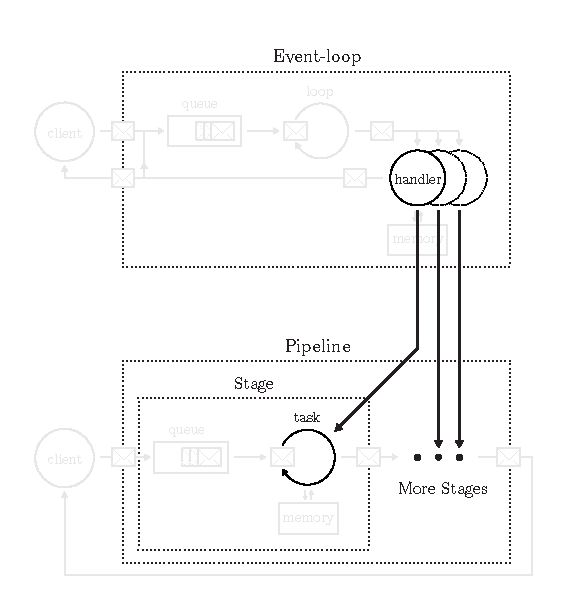
\includegraphics[width=\linewidth]{../resources/run-equivalence.pdf}
    \caption{Equivalence between handlers and tasks}
    \label{fig:run-equivalence}
  \end{minipage}
  \hfill
  \vrule
  \hfill
  \begin{minipage}[t]{0.45\textwidth}
    \centering
    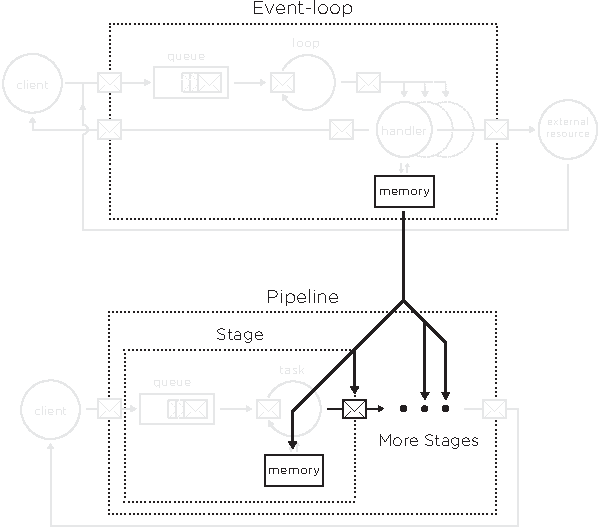
\includegraphics[width=\linewidth]{../resources/mem-equivalence.pdf}
    \caption{Distribution of the global memory abstraction with message passing}
    \label{fig:mem-equivalence}
  \end{minipage}
\end{figure}



% The invariance holds for the whole memory during the execution of each callback.
% As I explained in the previous section, this invariance is required to allow the concurrent execution of the different tasks.
% On the other hand, the invariance is explicit in the pipeline architecture, as all the stages have isolated memories.
% The coordination between these isolated process is made explicit by the developer through message passing.

% I argue that the state coordination between the callbacks requireing a global memory could be replaced by the message passing coordination used manually in the pipeline architecture.
% I argue that not all applications need concurrent access on the state, and therefore, need a shared memory.
% % Specifically, I argue that each state region remains roughly local to a stage during its modification.
% \nt{TODO review that, I don't know how to formulate these paragraphs. Identify the state and the data in the global memory.}

% \subsubsection{Transformation}

% This equivalence should allow the transformation of an event loop into several parallel processes communicating by messages.
% In this thesis, I study the static transformation of a program, but the equivalence should also hold for a dynamic transformation.
% I present the analyzis tools I developed to identify the state and the data from the global memory.
